\documentclass{article}
\usepackage{fullpage}
\usepackage{amsmath,amssymb}
\usepackage{amsthm}
\usepackage{graphicx}

\newcommand{\E}{\mathbb{E}}
\renewcommand{\P}{\mathbb{P}}
\newcommand{\calS}{\mathcal{S}}  % set of states
\newcommand{\calT}{\mathcal{T}}  % set of transition triples
\newcommand{\nA}{\mbox{A}}  % nucleotides:
\newcommand{\nC}{\mbox{C}}
\newcommand{\nG}{\mbox{G}}
\newcommand{\nT}{\mbox{T}}
\newcommand{\join}{\oplus}  % matches
\newcommand{\st}{\colon}  % such that
\newcommand{\var}{\mathop{\mbox{var}}}
\newcommand{\cov}{\mathop{\mbox{cov}}}

\theoremstyle{plain}
\newtheorem{theorem}{Theorem}
\theoremstyle{definition}
\newtheorem{example}{Example}[section]

\begin{document}

\section*{Introduction}

Interacting particle systems with neighborhood structure: transition probabilities generally not expressable (except TASEP).
Markov random fields with Glauber dynamics a case of this.

Example: Ising model.

Context-dependent substitution processes are an example of interest for phylogenetics and evolutionary inference.
Usually dealt with either by using larger and larger windows (but, only up to four bp),
or by doing MCMC over additional information (entire history of changes).
Also, Markov-along-the-genome method.

The difficulty comes from the fact that the rates of change at any one site depend in principle on arbitrarily far away sites,
so transition matrix is ginormous.

Goal: parameter inference, given before-after observations, or else observations descended from a common ancestor.

Review stats lit, e.g. reviews by Friel, original by Besag (autologistic model), genetics by Larribe and Fearnead.

Here restrict to one-dimensional neighborhood structure,
to make it easier.

\section{Notation and Examples}

The common framework of the above examples is a one-dimensional grid of $n$ sites,
and each site is labeled with one of a finite set of states.
These change with time -- so, write $X_i(t)$ for the state of the $i^\mathrm{th}$ site at time $t$,
where each $X_i(t) \in \calS$, the set of possible states.
(To avoid edge effects, we sometimes arrange these sites in a circle, so the indices are interpreted $\mod n$.)
The time evolution is Markov, and is determined by a set of transition rates and associated patterns.  
``Patterns'' are sequences of states, and we let $|u|$ denote the length of the pattern $u$.
Transition rates are assumed to be local and homogeneous, so for example saying ``pattern $u$ changes to $v$ at rate $\mu$''
means that if $(X_i(t), \ldots, X_{i+\ell}(t)) = (u_1, \ldots, u_\ell)$ (where $\ell=|u|=|v|$),
then $\P\{(X_i(t+dt), \ldots, X_{i+\ell}(t+dt)) = (v_1, \ldots, v_\ell) = \mu dt + o(dt)$,
regardless of the location $i$ along the sequence.
If more than one pattern would match to cause the same change, their rates add.
We call such a $(\mu,u,v)$ a ``transition triple''.
The set of all transition triples $\calT = \{ (\mu^j,u^j,v^j) \}_{j=1}^{n_T}$ 
determines the time evolution of the process.

It will often be convenient, notationally and computationally, to avoid edge effects
by treating the $n$ sites as a circle, and treating all indices $\mod n$.

\begin{example}[TASEP]
  The \emph{Totally Asymmetric Simple Exclusion Process} labels each site as ``empty'' or ``occupied'' (0 or 1, respectively), 
  and says that each occupied site, independently at rate $\lambda$, checks the site to the right to see if it is empty,
  and if it is, moves there.  
  This process therefore has only one transition triple:

  \begin{center}
    \begin{tabular}{c@{\quad$\to$\quad}c@{\quad at rate\quad }c}
      $u$  &  $v$  &  $\mu$  \\
      \hline
      01  &   10   &  $\lambda$
    \end{tabular}
  \end{center}

  This only has one parameter, the speed.  
  Note, however, that it may not be entirely trivial to estimate the speed,
  since (on the circle) it may not be obvious which particle moved where.

\end{example}

\begin{example}[CpG mutation]
  A sequence of genome can be written using A, C, G, and T;
  in the most general model of single-site mutation, each of the 12 possible transitions occurs at its own rate.
  Furthermore, it is a well-known observation that in many species, and certain contexts, 
  a C followed by a G has an additional, higher rate with either the C changing to a T or the G changing to an A.
  This simplest model of context-dependent substitution rates in a genome sequence has rates

  \begin{center}
    \begin{tabular}{c@{\quad$\to$\quad}c@{\quad at rate\quad }cc}
      $u$  &  $v$  &  $\mu$  & \\
      \hline
      $x$  &  $y$  &  $m_{xy}$ & \qquad $x \neq y \in \{\nA,\nC,\nG,\nT\}$  \\
      CG   &  TG   &  $\gamma$ & \\
      CG   &  CA   &  $\gamma$ &  
    \end{tabular}
  \end{center}

  This has 13 parameters.
  Note that there are no conserved quantities here, unlike in TASEP,
  which we could imagine as indestructible particles moving.


\end{example}


\begin{example}[Ising model with Glauber dynamics]
  In the Ising model, each site is labeled as either ``up'' or ``down'' ($+1$ or $-1$ respectively),
  imagined as magnetic dipoles,
  and the energy associated with a given state $x$ is $H(x) = - \beta \sum_i x_i x_{i+1} - \gamma \sum_i x_i$.
  The associated stationary distribution on configurations is proportional to $\exp(-H(x))$.
  One way to add temporal dynamics that preserve the distribution 
  is to say that each site, independently at rate $\lambda$,
  forgets its spin, 
  and reconfigures to a state chosen with probability proportional to the stationary probability of the resulting configuration.
  This is known as ``Glauber dynamics'', and ignoring transitions that don't change the state,
  we get that if patterns $u$ and $v$ differ at only one site, then $u$ changes to $v$ at rate $1/(1+\exp(H(u)-H(v)))$, so

  \begin{center}
    \begin{tabular}{c@{\quad$\to$\quad}c@{\quad at rate\quad }c}
      $u$  &  $v$  &  $\mu$  \\
      \hline
      $+++$  &   $+-+$   &  $\lambda/1+e^{2\beta - \gamma})$ \\
      $++-$  &   $+--$   &  $\lambda/(1+e^{-\gamma})$ \\
      $+-+$  &   $+++$   &  $\lambda/(1+e^{-2\beta + \gamma})$ \\
      $+--$  &   $++-$   &  $\lambda/(1+e^{\gamma})$ \\
      $-++$  &   $--+$   &  $\lambda/(1+e^{-\gamma})$ \\
      $-+-$  &   $---$   &  $\lambda/(1+e^{-2\beta - \gamma})$ \\
      $--+$  &   $-++$   &  $\lambda/(1+e^{\gamma})$ \\
      $---$  &   $-+-$   &  $\lambda/(1+e^{2\beta + \gamma})$ 
    \end{tabular}
  \end{center}

  This has three parameters: the speed $\lambda$, the inverse temperature $\beta$, and the strength of magnetization $\gamma$
  (here scaled by temperature).

\end{example}


\paragraph{The generator matrix}
For clarity, we should define how the set of transition rates determines the transition rate matrix,
the $|\calS|^n \times |\calS|^n$ matrix $G(n)$ whose $(x,y)^\text{th}$ entry gives the instantaneous rate 
with which the process in state $x$ jumps to state $y$.
% Let $x_i^{(\ell)} = (x_i, x_{i+1}, \ldots, x_{i+\ell-1})$ be the subsequence of length $\ell$ beginning at location $i$, and 
For each $1\le i \le n$, pattern length $\ell \ge 0$, and patterns $u,v \in \calS^\ell$ define the relation
\[
x \xrightarrow{i,u,v} y \qquad \text{iff} \qquad \begin{cases}
  x_k = y_k \quad &\text{for } k<i \\
  x_{i+k} = u_k \quad &\text{for } 0 \le k < \ell \\
  y_{i+k} = v_k \quad &\text{for } 0 \le k < \ell, and \\
  x_k = y_k \quad &\text{for } k\ge i+\ell ,
\end{cases}
\]
i.e.\ if $x$ and $y$ match except for in $i,i+1,\ldots,i+\ell-1$, where $x$ matches with $u$ and $y$ matches with $v$.
(Interpet these indices modulo $n$, even for short sequences, a point we will come back to.)
We'll also need the set of defined transitions in $\calT$ 
that can move from $x$ to $y$ at a given location: let  $J(i,x,y) = \{ (\mu^j,u^j,v^j) \in \calT \st x \xrightarrow{i,u^j,v^j} y \}$.
Then, the rate $G(n)_{x,y}$ is the sum of all matching transition rates,
namely
\begin{align} \label{eqn:G_defn}
  G(n)_{x,y} = \sum_{i=1}^n \sum_{J(i,x,y)}  \mu^j ,
\end{align}
and if there are no triples $(\mu,u,v)$ with $x \xrightarrow{i,u,v} y$ for some $i$, then $G(n)_{x,y}=0$.
This is just to say that the transition rate from $x$ to $y$ is the sum of the mutation rates of all transition triples
that could change $x$ into $y$.
In principle, this gives us the transition probabilities for the process:
\begin{align} \label{eqn:full_likelihood}
    p_n(t;x,y) := \P\{ X(t) = y \mid X(0) = x \} = (e^{tG(n)})_{xy} .
\end{align}


\section{Simulation}

First, it will be useful to have a brief description of how to simulate such a process.
Briefly, we can put down a Poisson process of times and locations of possible changes,
at an appropriate rate $\mu_*$,
and then resolve each possible change in temporal order.
We situate ``changes'' at the beginning of the matching pattern,
so $\mu_*$ can be defined as the maximum sum of rates matching  the start of a sequence:
\[
\mu_* = \max \left\{ \sum_{y \in \calS^n} \sum_{j\in J(1,x,y)} \mu_j \st x \in \calS^n \right\} .
\]
Now sample possible changes: let $s_{ij}$ denote the $j^\text{th}$ possible change at site $i$,
so that $0 \le s_{i1} < s_{i2} < \cdots < s_{iN_i} \le t$ is a rate $\mu_*$ Poisson process.
Then, suppose we have determined the state at time $s$ to be $X(s) = x$,
and the next event is $s_{ij} = \min \{ s_{k\ell} : s_{k\ell}>s \}$.
The process then jumps to a new state at times $s_{ij}$ with probability proportional to the corresponding rate.
In other words, let
\[
q_k = \begin{cases}
  \mu_k/\mu_* \qquad & \text{if } x_i^{(|u_k|)} = u_k  \\
  0 \qquad & \text{otherwise,}
\end{cases}
\]
and let $q_0 = 1-\sum_{k=1}^{n_T} q_k$.
By construction of $\mu_*$, $q_0\ge 0$.)
Now choose transition $k$ with probability $q_k$, and if $k>0$, replace $x_i^{|u_k|}$ with $v_k$.

For instance, to simulate TASEP, one has only to let $\mu_*=\lambda$, and at each $s_{ij}$
check if at site $i$ there is a 1 followed by a 0,
and if so, switch them.


\section{Inference}

The problem at hand is to infer the parameters of the model, given the state at time 0 and later at time $t$.
If $n$ is large enough and $t$ is not too large,
this should be feasible.
(If $t$ is too large, the process may ``saturate'' --
if there are many changes at most sites, then in at least most models, 
we will lost most of the information about the dynamics,
retaining information only about the parameters that affect the stationary distribution.
In TASEP, we lose all information as it approaches stationarity,
in the Ising model we have information about $\beta$ and $\gamma$ but not $\lambda$,
and in the CpG model it is not immediately clear.


But, how can we extract the information?
These are Markov processes, on the state space $\calS^n$, 
so the full likelihood function is given by \eqref{eqn:full_likelihood},
but doing anything with the $|\calS|^n \times |\calS|^n$ matrix $G_n$ is clearly infeasible.
We can, however, compute \eqref{eqn:full_likelihood} for smaller $n$,
so the first thing that one might think to do is to break the sequence up into many blocks of length $m$,
and treat these as independent, taking $m$ as large as is feasible.
Then we would define $p_m(t;x,y)$ to be the probability that a string $x$ of length $m$ evolves to string $y$ over time $t$,
denote by $x_i^{(m)}$ the block of length $m$ beginning at index $i$,
and obtain the approximate likelihood function
\[
  \prod_{k=0}^{n/m} p_m(x_{km}^{(m)},y_{km}^{(m)}) .
\]
Variations are possible (what do we do about the edge effects for $p_m$?),
but in any case there is no guarentee that this is close to correct,
as it ignore dependencies between neighboring blocks.

Intuitively, we want to increase the size of the context 
-- but increasing $m$ does not do this, as there are always edge effects.
However, we could look at the context in the initial sequence but not in the final sequence,
including the states of an additional $\ell$ and $r$ sites on the left and right, respectively.
Concretely, define the marginal probabilities
\begin{align}
  p_{\ell,m,r}(t;x,y) &= \sum_{a \in \calS^\ell} \sum_{b \in \calS^r} p_{\ell+m+r}(t;x,a \join y \join b) , \quad \text{for}\; x \in \calS^{\ell+m+r}, \; y \in \calS^m ,
\end{align}
where $a \join y \join b$ is the sequence composed of concatenating $a$, $y$, and $b$ together in that order.
This is the probability that if we begin with a sequence $x$ of length $\ell+m+r$, 
then after time $t$ we will see at the middle $m$ positions the pattern $y$,
ignoring what is present in the leftmost $\ell$ and rightmost $r$ positions.
In a long sequence, $p_m(x,z)$ might not be a very good approximation for $\P\{ X_i^{(m)}(t) = z | X_i(0)^{(m)} = x \}$,
we do expect $p_{\ell,m,r}(x,y)$ to be correct, asymptotically in $\ell$ and $r$:
\begin{align} \label{eqn:window_approx}
  \P\{ X_i^{(m)}(t) = y | X_i(0)^{(\ell+m+r)} = x \} \approx p_{\ell,m,r}(x,y) .
\end{align}
We provide a concrete statement of this approximation later.

%%%%
\subsection{Summary statistics}

Now we know how to compute the (marginal) probability that a particular subsequence changes into another subsequence.
For patterns $x$ and $y$, with offset $\ell$ (so that $|x|=|y|+2\ell$),
we can count how many times $x$ appears in $X(0)$,
and how many times $x$ appears in $X(0)$ while $y$ appears at the same place in $X(t)$, offset by $\ell$.
For instance, if $x$ is ACTCAC, $y$ is CGC, and $\ell=3$, this looks like:
\begin{center}
\begin{tabular}{c|ccccccc}
 $x$ &  C  & A & C & T & C & A & C \\
 $y$ &  $\centerdot$  & $\centerdot$  & C & G & C & $\centerdot$  & $\centerdot$  
\end{tabular}
\end{center}
where $\cdot$ could be any base.
Let $N(x)$ and $N_\ell(x,y)$ count these events, respectively.

From the definitions above, 
the expected number of times $y$ would appear juxtaposed with $x$ is approximately $N(x)p_{\ell,m,r}(x,y)$.
Covariances are also easy to compute.
If we define $M_i(x,y)$ to be 1 if $X_{i-\ell}^{|x|}(0)=x$ and $X_i^({|y|})(t)=y$, and 0 otherwise,
so that $N(x,y) = \sum_{i=1}^n M_i(x,y)$, then
\begin{align}
  \var[N(x,y)] &= \sum_{i=1}^n \var[M_i(x,y)] + \sum_{i\neq j} \cov[M_i(x,y), M_j(x,y)] \\
  &= n \var[M_1(x,y)] + 2n\sum_{k=1}^n \cov[M_1(x,y),M_{k+1}(x,y)] \\
  &\approx n p_{\ell,m}(x,y)(1-p_{\ell,m}(x,y)) + 2n\sum_{k=1}^{m+2\ell} \left( \E[M_1(x,y) M_{k+1}(x,y)] - p_{\ell,m}(x,y)^2 \right) \\
  &= n p_{\ell,m}(x,y)(1-(1+2m+4\ell)p_{\ell,m}(x,y)) + 2n\sum_{k=1}^{m+2\ell} \E[M_1(x,y) M_{k+1}(x,y)] .
\end{align}
The term $\E[M_1(x,y) M_{k+1}(x,y)]$ is the probability that $x$ matches at both site 1 and site $k+1$,
and that $y$ matches both at site $\ell+1$ and at site $\ell+k+1$.
For this to be nonzero, the joint pattern $(x,y)$ must allow self-overlaps.
Similarly, if $(x_1,y_1) \neq (x_2,y_2)$ then
\begin{align}
  \begin{split}
    \cov[N(x_1,y_1),N(x_2,y_2)] 
    & \approx - n (2m+4\ell) p_{\ell,m}(x_1,y_1)p_{\ell,m}(x_2,y_2) \\
    & \qquad {} + n\sum_{k=1}^{m+2\ell} \E[M_1(x_1,y_1) M_{k+1}(x_2,y_2) + M_1(x_2,y_2) M_{k+1}(x_1,y_1)] .
  \end{split}
\end{align}


%%%%
\subsection{A likelihood function}

The covariance calculations show that
if $p_{\ell,m}(x,y)$ is small enough (i.e.\ the pattern is not common),
then $N(x,y)$ is close to Poisson.
Using this observation, we can estimate parameters by composite likelihood,
using all $N(x,y)$ as data.
Maximum likelihood then gets an asymptotically unbiased estimate of the parameters.
However, since they are not independent, to get confidence intervals, we need to either simulate, or do something different.

If we use only a subset of patterns $\{(x_k,y_k)\}$ chosen so that $\E[M_1(x,y) M_{k+1}(x,y)]$ is small (or zero),
the entire collection $\{N(x_k,y_k)\}$ will be close to independent Poisson.
(using Stein's method)
Then we'll have the correct likelihood function for (this subset of) data.
If changes are rare, then one way to get a set of patterns with this property is to only choose ones such that going from $x$ to $y$ entails a change;
and any overlapping patterns must require additional changes, 
i.e.\ if $(x_1,y_1)$ matches at $i_1$, 
then for $(x_2,y_2)$ to match at $i_2$, 
there must be additional changes outside $(i_1,\ldots,i_1+\ell-1)$.

Here is one way to obtain such a set.
Take a pair of patterns $(x,y)$, that overlap at $m$ positions,
and suppose that they differ at $1 \le i_1, \ldots, i_d \le m$.
For example, in the example above with $m=3$ and $\ell=2$,
\begin{center}
\begin{tabular}{c|ccccccc}
 $x$ &  C  & A & C & T & C & A & C \\
 $y$ &  $\centerdot$  & $\centerdot$  & C & G & C & $\centerdot$  & $\centerdot$  
\end{tabular}
\end{center}
$x$ and $y$ differ only at (relative) position $i_1=2$.
Let $\bar i = (1/d) \sum_{j=1}^d i_j$ be the mean position of the changes,
and take only patterns with $(m-1)/2 < \bar i \le (m+1)/2$.
As another example,
\begin{center}
\begin{tabular}{c|ccccccc}
 $x$ &  A & C & T & C & A & C & G \\
 $y$ &  $\centerdot$  & $\centerdot$  & G & C & A & $\centerdot$  & $\centerdot$  
\end{tabular}
\end{center}
has $i_1 = \bar i = 1$.
No two such patterns can be shifted versions of each other
without adding more changed sites,
since shifting by $k$ without adding changed sites just adds $k$ to $\bar i$.



%%%%
\subsection*{Proof of the approximation}

\begin{proof}

In fact, the approximation improves exponentially as $\ell$ and $m$ increase --
here is a simple argument.
Suppose the maximum length of any transition pattern is $R = \max\{ |u| : (\mu,u,v) \in \calT \}$.
The transition rate at site $i$ at time $s$ is determined if we know $X_{i-R}^{(2R+1)}(s)$;
this can be determined from $X_{i-R}^{2R+1}(0)$ and the outcome of all changes happening before time $s$ at sites in $(i-R-1, \ldots, i+R)$.
These will depend in turn on the outcome of previous possible changes.
For each site $i$ and times $s_1 < s_2$, define the set of states $H(i,s_1,s_2)$ 
so that if one knows the possible change points $s_{ij}$,
then changes outside of $H(i,s_1,s_2)$ do not affect the distribution of $X_i(s_2)$.
Concretely, define $H(i,s_1,s_2)$ by the property that $i \in H(i,s_1,s_2)$, and
\begin{gather}
  \text{if } s_1 < s_{jk} \le s_2 \text{ for some } i-R-1 \le j \le i+R, \text{ then } H(j,s_1,s_{jk}) \subseteq H(i,s_1,s_2) .
\end{gather}
In other words, $H(i,s_1,s_2)$ is the union of the $R$-neighborhoods of $i$ and all possible changes occurring in $H(i,s_1,s_2)$ between $s_1$ and $s_2$.
For a set of states $I$, let $H(I,s_1,s_2) = \bigcup_{i\in I} H(i,s_1,s_2)$.
Formally, the state $X_i(s_2)$ is conditionally independent of $\{X_j(s_1) \st j \notin H(i,s_1,s_2)\}$.
Informally, the approximation \eqref{eqn:window_approx} will be good if $H$ does note expand beyond the flanking context.
Now, MAKE THIS EASIER TO READ
\begin{multline}
  \P\{ X_i^{(m)}(t) = y \mid X(0) \} 
  = \P\left\{ H(\{i,\ldots,i+m\},0,t)\subseteq\{i-\ell,\ldots,i+m+r\} \right\} \\
   \qquad \qquad {} \times \P\left\{ X_i^{(m)}(t) = y \mid X_{i-\ell}^{(\ell+m+r)}(0), \; H(\{i,\ldots,i+m\},0,t)\subseteq\{i-\ell,\ldots,i+m+r\} \right\} \\
     \qquad {} + \P\left\{ H(\{i,\ldots,i+m\},0,t)\nsubseteq\{i-\ell,\ldots,i+m+r\} \right\}  \\
   \qquad\qquad {} \times \P\left\{ X_i^{(m)}(t) = y \mid X_{i-\ell}^{(\ell+m+r)}(0), \; H(\{i,\ldots,i+m\},0,t)\nsubseteq\{i-\ell,\ldots,i+m+r\} \right\} ,
\end{multline}
and so
\begin{align} \label{eqn:prob_approx}
  \left| \P\{ X_i^{(m)}(t) = y \mid X(0) \} - p_{\ell,m,r}(t;x,y) \right| \le 2 \P\left\{  H(\{I,\ldots,i+m\},0,t)\subseteq\{i-\ell,\ldots,i+m+r\} \right\}.
\end{align}

So, the error is bounded by the probability that $H(I,0,t)$ is larger than the context from $I-\ell$ to $I+r$.
However, following $H$ backwards in time, the outer edge of $H$ expands as a continuous-time random walk:
for instance, the left edge $L(s) = \min \{ j \in H(I,t-s,t) \}$ jumps leftwards at rate $R\mu_*$ with a random jump size
that has mean $R/2$.
General facts about random walks imply that \eqref{eqn:prob_approx} is bounded above by $C e^{-\alpha \ell/t}$, for some constants $C$ and $\alpha$.

\end{proof}

%%%%%%%%
\subsection{Edge effects and cyclicization}

The choice to treat long sequences as cyclical is generally of little importance.
However, we have defined in \eqref{eqn:G_defn} the basic building block of our approximation, $G(m)$,
to be the transition matrix \emph{for a circular sequence} of length $m$, where $m$ may be short.
This seems strange -- but, what else would we do at the edges?
We want to use $G(\ell+m+r)$ to compute the chance that a given $(\ell+m+r)$-sequence ends up with another given $m$-sequence in the middle;
and if $\ell$ and $r$ are big enough relative to $t$, this will be a good approximation regardless of what we do at the edges.
One answer would be to not allow patterns hanging off of either end to match,
resulting in a slight underestimate of the chance of change.
A better approximation would be to use the marginal frequencies in some way to average over surroudning sequence 
-- but, this requires marginal frequencies to be known, and these are not stationary.
However, the leftmost site in a randomly chosen window is a sample from the marginal distribution,
and if sites separated by distance $\ell+m+r$ are sufficiently uncorrelated,
wrapping the sequence around is a good approximation to averaging over marginal frequencies in the surrounding sequence.
It is easy to imagine situations where this would not be the best solution --
but again, if $\ell$ and $r$ are large enough, it won't matter much.

%%%%%%%%
\section{Phylogenetic inference}

In phylogenetic applications, rather than ``before'' and ``after'' observations,
we get two (or more) observations evolved from a common root.
In the simplest case of two taxa we have two processes $X$ and $Y$,
with identical starting states $X(0)=Y(0)$,
observed only at times $t_X$ and $t_Y$ respectively.

If the approximation described above holds,
then we can write the probability that we see (long) pattern $x$ in $X(t_X)$ juxtaposed with (short) pattern $y$ in $Y(t_Y)$
using the pattern frequencies at the root.
Concretely: pick a random location $I$ in the sequence and let $X_{I-\ell}^{m+2\ell}(0) = \rho$ be the (long) pattern seen there at the root,
and write $\pi(z)$ for the frequency of pattern $z$ in $X(0)$, i.e.\ $\P\{\rho=z\}=\pi(z)$.
% Given the corresponding pattern in $X(t_X)$, the distribution of $\rho$ is proportional to
% \[
%     \P\{ \rho=z \mid X_{I-\ell}^{m+2\ell}(t_X)=x\} \propto \pi(z) p_{m+2\ell}(t,z,x) .
% \]
The probability that we see $x$ and $y$ at the random location $I$ is
\begin{align} \label{eqn:phylo_likelihood}
    \P\{X_{I-\ell}^{m+2\ell}(t_X)=x \text{ and } Y_I^\ell(t_Y)=y \} = \sum_{z \in \calS^{m+2\ell}} \pi(z) p_{m+2\ell}(t_X,z,x) p_{m,\ell}(t_Y,z,y) .
\end{align}
This can be computed without much more effort than the simpler case above,
given the frequencies at the root, as described in greater generality below.



%%%%
\subsection{The root distribution}

We clearly don't want to add an extra parameter $\pi(z)$ for all $z \in \calS^{m+2\ell}$. 
If nothing else, it would make the inference depend on $m$ and $\ell$, which we'd like to avoid.
One approach would be to put a Dirichlet distribution on $\pi(z)$.
This has the nice property that you can choose priors that are consistent across different values of $m$ and $\ell$.
We'd have to still MCMC around in the space of $\pi(z)$, so they'd be nuisance parameters from that point of view.
Also, making the frequencies at the root random introduces correlations between counts, which we want to avoid.
An alternative is to specify $\pi$ through lower-dimensional statistics,
for instance to model the root state as a sample from a Markov random field
with parameters for the marginal frequencies of each state, and pairwise (or higher) correlations between them.

A Markov random field with interactions between sites no more than distance two away 
is determined by the energy function $\phi(a,b,c)$ which gives the ``energy'' of the configuration $abc$ for each $a,b,c \in \calS$.
We use this to define the distribution on root patterns $\pi$ by
\begin{align}  \label{eqn:root_mrf}
    \pi(z) = \frac{1}{Z} \exp\left( - \sum_{i=1}^{|z|} h(z_{i-1},z_i,z_{i+1}) \right),
\end{align}
i.e.\ the exponential of the total energy of each three adjacent sites,
where $Z$ is the normalizing constant.
Note that it is often difficult to compute $Z$ in applications of Markov random fields,
but here we are working with relatively short sequences, 
so we just compute \eqref{eqn:root_mrf} for all possible $z$, and divide by the sum.
(However, for this same reason this is not equivalent to saying that $X(0)$ is a sample from the Markov random field
and finding the distribution of patterns within this.)


%%%%%
\subsubsection{Mixing}

There can be significant confounding of the frequencies at the root with the other parameters,
which results in poor mixing.
(See CpG results, below.)
To see why this is, consider the following back-of-the-envelope calculation.
Take $x \neq y$ to be single bases (so, set $\ell=0$ and $w=1$),
so that $N(x,y)$ gives the number of times an $x$ and a $y$ are homologous.
Let $q(x,y)$ be the instantaneous rate that $x \to y$ (averaged somehow over context?),
so that $N(x,y)$ should be, roughly,
\begin{align*}
  \sum_z \pi(z) q(z,x) q(z,y) &\approx t \pi(x) (1+q(x,x)) q(x,y) + t \pi(y) q(y,x) (1+q(y,y)) ,  
\end{align*}
where as usual $q(x,x) = (-1) \sum_{z \neq x} q(x,z)$ is (minus) the total jump rate out of $x$.

So, when we propose a change to $\pi$ we might want to also adjust the rates accordingly to keep this more-or-less constant:
if we chnage $\pi(x) \mapsto \pi(x) + \epsilon_x$, we want $\delta_{xy}$ to satisfy
\begin{align*}
  \sum_z \pi(z) q(z,x) q(z,y) = \sum_z (\pi(z) + \epsilon_z) ( q(z,x) + \delta_{zx} ) ( q(z,y) + \delta_{zy} ) ,
\end{align*}
or, to first order in $\delta$,
\begin{align*}
  0 &\approx \sum_z \epsilon_z q(z,x) q(z,y) + \sum_z \pi(z) \delta_{zx} q(z,y) + \sum_z \pi(z) q(z,x) \delta_{zy} \\
   &\approx \sum_z \epsilon_z q(z,x) q(z,y) + \sum_z (\pi(z)+\epsilon_z) \delta_{zx} q(z,y) + \sum_z (\pi(z)+\epsilon_z) q(z,x) \delta_{zy} \\
   &\approx \epsilon_x (1+q(x,x)) q(x,y) + \epsilon_y q(y,x) (1+q(y,y)) + (\pi(y)+\epsilon_y) \delta_{yx} (1+q(y,y)) + (\pi(x)+\epsilon_x) (1+q(x,x)) \delta_{xy} \\
   &= \left( \epsilon_x q(x,y) + (\pi(x)+\epsilon_x) \delta_{xy} \right)(1+q(x,x)) + \left( \epsilon_y q(y,x) + (\pi(y)+\epsilon_y) \delta_{yx} \right)(1+q(y,y)) 
\end{align*}
One solution to this is to let $\delta_{xy} = - \epsilon_x q(x,y) / \pi(x)$.

Suppose each change is a single-base change, so that changes $\delta \mu_i$ in $\mu$ contribute to $q$ by
$\delta_{xy} = \sum_{i: x \to y} \delta \mu_i$.
Given $\delta_{xy}$, this gives a linear equation for $\delta \mu_i$ that may or may not be solvable,
but certainly is if we have all the single-base transitions as paramters.

%%%%%%%%%%%
\section{Computation}

For inference, we need to compute the $|\calS|^{m+2\ell} \times |\calS|^m$ matrix whose $(x,y)^\text{th}$ entry is $p_{m,\ell}(t,x,y)$,
for various $t$.
This matrix is a projection of the $|\calS|^{m+2\ell} \times |\calS|^{m+2\ell}$ matrix whose $(x,z)^\text{th}$ entry is
\begin{align}
    p_{m+2\ell}(x,z) = \left( e^{t G(m+2\ell)} \right)_{x,z} ,
\end{align}
where $G(m+2\ell)$ is the sparse $|\calS|^{m+2\ell} \times |\calS|^{m+2\ell}$ matrix defined in \eqref{eqn:G_defn}.
The ``projection'' we need just marginalizes over long patterns $z$ that match the shorter pattern $y$:
if we define the matrix $U$ in this way, so that $U_{zy}=1$ if $z_\ell^m=y$ and $U_{zy}=0$ otherwise,
then
\[
    p_{m,\ell}(t,x,y) = \sum_{z \in \calS^{m+2\ell}} \left( e^{t G(m+2\ell)} \right)_{xz} U_{zy} ,
\]
so in fact we don't need the entire matrix $e^{t G(m+2\ell)}$,
just the product of this matrix with each of the columns of $U$.

Modern techniques in sparse matrix computation (Krylov methods) provide efficient ways to do this
by only multiplying $G$ and $U$ some number of times, 
which is much more efficient because $G$ is sparse.

\subsection{Updating $G$}

We can also take advantage of the sparsity of $G$ to perform efficient computation of the likelihood
under many sets of parameters.
First note that $G(m+2\ell)$ has, assuming only single-position changes,
$(1+m(|\calS|-1)) |\calS|^{m+2\ell}$ nonzero entries, since each of the $|\calS|^{m+2\ell}$ can change in $m$ places.
This will determine how the computation scales with $m$, $\ell$, and $|\calS|$,
once we precompute a number of things.
Let $g = (g_1, \ldots, g_d)$ be the nonzero entries of $G$, in some fixed ordering;
sparse matrix representations of $G$ store only $g$ along with information about the rows and columns these are found in.
Each $g_i$ is a linear combination of mutation rates $\mu_j$, say $g_i = \sum_j a_{ij} \mu_j$;
so by precomputing $a_{ij}$ we can efficiently update $G$.
This is true if the boundary conditions are circular, mean-value, or neither.

We can do similar precomputations to help with the case of selective differences:
XXX describe


\subsection{Phylogenetic peeling}

Furthermore, note that the further calculations in the phylogenetic case can be done using these methods.
To compute
\[
    \sum_z \pi(z) p_{m+2\ell}(t_X,z,x) p_{m,\ell}(t_Y,z,y) 
    = \sum_z \left( e^{t_X G(m+2\ell)} \right)_{zx} \pi(z) \sum_w \left( e^{t_X G(m+2\ell)} \right)_{zw} U_{wy} ,
\]
we can first compute $\sum_w \left( e^{t_X G(m+2\ell)} \right)_{zw} U_{wy}$ as above,
multiply by $\pi(z)$, and then apply the algorithm again using the transpose of $G(m+2\ell)$.

Using the R package expm, this makes computation quite feasible:
with four possible states and $\ell=2$ and $m=1$, so that $G(m+2\ell)$ is a $1024 \times 1024$ matrix,
computing $e^{t G(5) }$ takes 13 seconds, while computing $e^{t G(5)} U$ takes only 0.3 seconds.
Increasing to $\ell=4$ and $m=1$ or $\ell=3$ and $m=2$ is still feasible, taking $e^{t G(8)} U$ in 42 and 47 seconds, respectively
(and much longer for the whole matrix $e^{t G(8)}$).

More generally\dots

\begin{center}
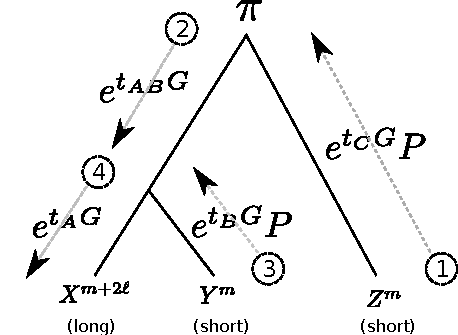
\includegraphics{peeling-schematic}
\end{center}

To compute the likelihood on a more complicated tree, consider the following,
with the three-taxon tree above as an example,
where we are counting occurrences of (long) $m+2\ell$-tuples in taxon $X$,
and (shorter) $m$-tuples in taxa $Y$ and $Z$.

We can compute the likelihood in a similar way, summing over the root state (the summation over $u$)
and the interior node ($v$):
\begin{align} \label{eqn:three_taxa_likelihood}
  \begin{split}
    & \P\{X_{I-\ell}^{m+2\ell}=x \text{ and } Y_I^\ell=y \text{ and } Z_I^\ell=z \} \\
    &\qquad = \sum_{u \in \calS^{m+2\ell}} \pi(u) p_{m,\ell}(t_C,u,z) \sum_{v \in \calS^{m+2\ell}} p_{m+2\ell}(t_{AB},u,v) p_{m+2\ell}(t_{A},v,x) p_{m,\ell}(t_B,v,y) 
  \end{split}
\end{align}
The steps for computing this are then:
\begin{enumerate}

  \item Compute $M_1(u,z) = p_{m,\ell}(t_C,u,z)$ (a $|\calS|^{m+2\ell} \times |\calS|^m$ matrix)

  \item Compute $M_2(v,z) = \sum_{v \in \calS^{m+2\ell}}  p_{m+2\ell}(t_{AB},u,v) \pi(u) M_1(u,z)$ (still a $|\calS|^{m+2\ell} \times |\calS|^m$ matrix)

  \item Compute $M_3(v,y) = p_{m,\ell}(t_B,v,y)$ (a $|\calS|^{m+2\ell} \times |\calS|^m$ matrix) 

  \item Compute $M_4(x,(y,z)) = \sum_{v \in \calS^{m+2\ell}} p_{m+2\ell}(t_{A},v,x) M_3(v,z) M_4(v,y)$ (stored as a $|\calS|^{m+2\ell} \times |\calS|^{2m}$ matrix).

\end{enumerate}
Then $M_4$ gives all the likelihoods.
This is depicted in the figure, writing $\left(e^{tG}\right)_{ab}$ for the matrix $p_{m+2\ell}(t,a,b)$,
and $P$ for the projection matrix that gives $p_{m,\ell}(t,a,b) = \left( e^{tG} P\right)_{ab}$.


In total there are $|\calS|^{3m+2\ell}$ possible data combinations.  
However, we can reduce dimensionality by replacing the last step with
\begin{enumerate}

  \item[4'.] Compute $M_4(x,w) = \sum_{v \in \calS^{m+2\ell}} p_{m+2\ell}(t_{A},v,x) M_3(v,w) M_4(v,w)$ (stored as a $|\calS|^{m+2\ell} \times |\calS|^{m}$ matrix).

\end{enumerate}
and only computing the likelihood for cases with $y=z=w$.
On a three-taxon tree it is not clear that this is desireable, since missing out on double transitions 
might be a significant loss of information,
but on larger trees it seems likely that we'd want to restrict to combinations with most sites agreeing across the tree.
(Note, however, that one should not first look at the data, observe which combinations $(y,z)$ were most common, and then restrict to only those!)




%%%%%%
\section{Bayesian things}

So, suppose we've got a list of patterns $(x_i,y_i)$
and we're happy with the idea that they're independent.
Recall that
\[
\E\left[ N(x,y) \mid N(x) \right] = N(x) p_{m,\ell}(x,y) ,
\]
Parameters $\theta$ enter implicitly through $p_{m,\ell}$.


In the case that we observe the initial sequence, $N(x,y)$ are binomial with sample size $N(x)$.
and so the likelihood is 
\[
\prod_x N(x)! \prod_y \frac{ p_{m,\ell}(x,y)^{N(x,y)} }{ N(x,y)! } ,
\]
and so the negative log likelihood is, up to a constant,
\[
\sum_{x,y} N(x,y) \log p_{m,\ell}(x,y) .
\]





%%%%%%%
\section{Simulation results}

The method works well to find point estimates of the parameters.
Obtaining posterior density estimates using the approximation likelihood function on a subset of patterns
works in some cases;
in other cases the likelihood surface is still too peaked, underestimating the uncertainty.

\subsection{TASEP}

Strings of length $10^5$ were evolved under TASEP for varying amounts of time,
and pattern occurrences counted.
Running 10,000 MCMC iterations with window sizes of $\ell=w=3$ (total length 9) on these takes around 40 minutes.
Apparently, the patterns used were not sufficiently independent in this case,
as the posterior is too sharp.

Here's a short example sequence with $\lambda=1$:
\begin{center}
 \setlength{\tabcolsep}{0pt}
\begin{tabular}{cccccccccccccccccccccccccccccccccccccccccccccccccccccccccccc}
X&X&X&O&O&X&O&O&O&O&X&O&X&O&X&X&O&O&X&O&O&X&O&X&X&X&O&X&O&O&O&X&X&O&X&O&O&O&X&X&O&O&O&X&O&O&O&O&X&O&X&X&O&X&X&O&O&X&O&O \\
$\centerdot$&O&X&O&X&O&O&O&X&$\centerdot$&O&X&O&O&X&X&X&o&x&$\centerdot$&o&O&X&x&x&O&X&O&X&o&o&O&X&X&$\centerdot$&$\centerdot$&o&o&O&X&X&o&$\centerdot$&O&X&$\centerdot$&o&o&$\centerdot$&$\centerdot$&O&X&X&x&O&X&o&O&X&$\centerdot$
\end{tabular}
\end{center}
here particles are X's, moving to the right; and spaces are O's; 
in the second line, 
$\centerdot$ is a position that has not considered a change; lowercase letters are positions that considered a change but did not;
and upper case are positions that did change.

\begin{figure}
  \begin{center}
    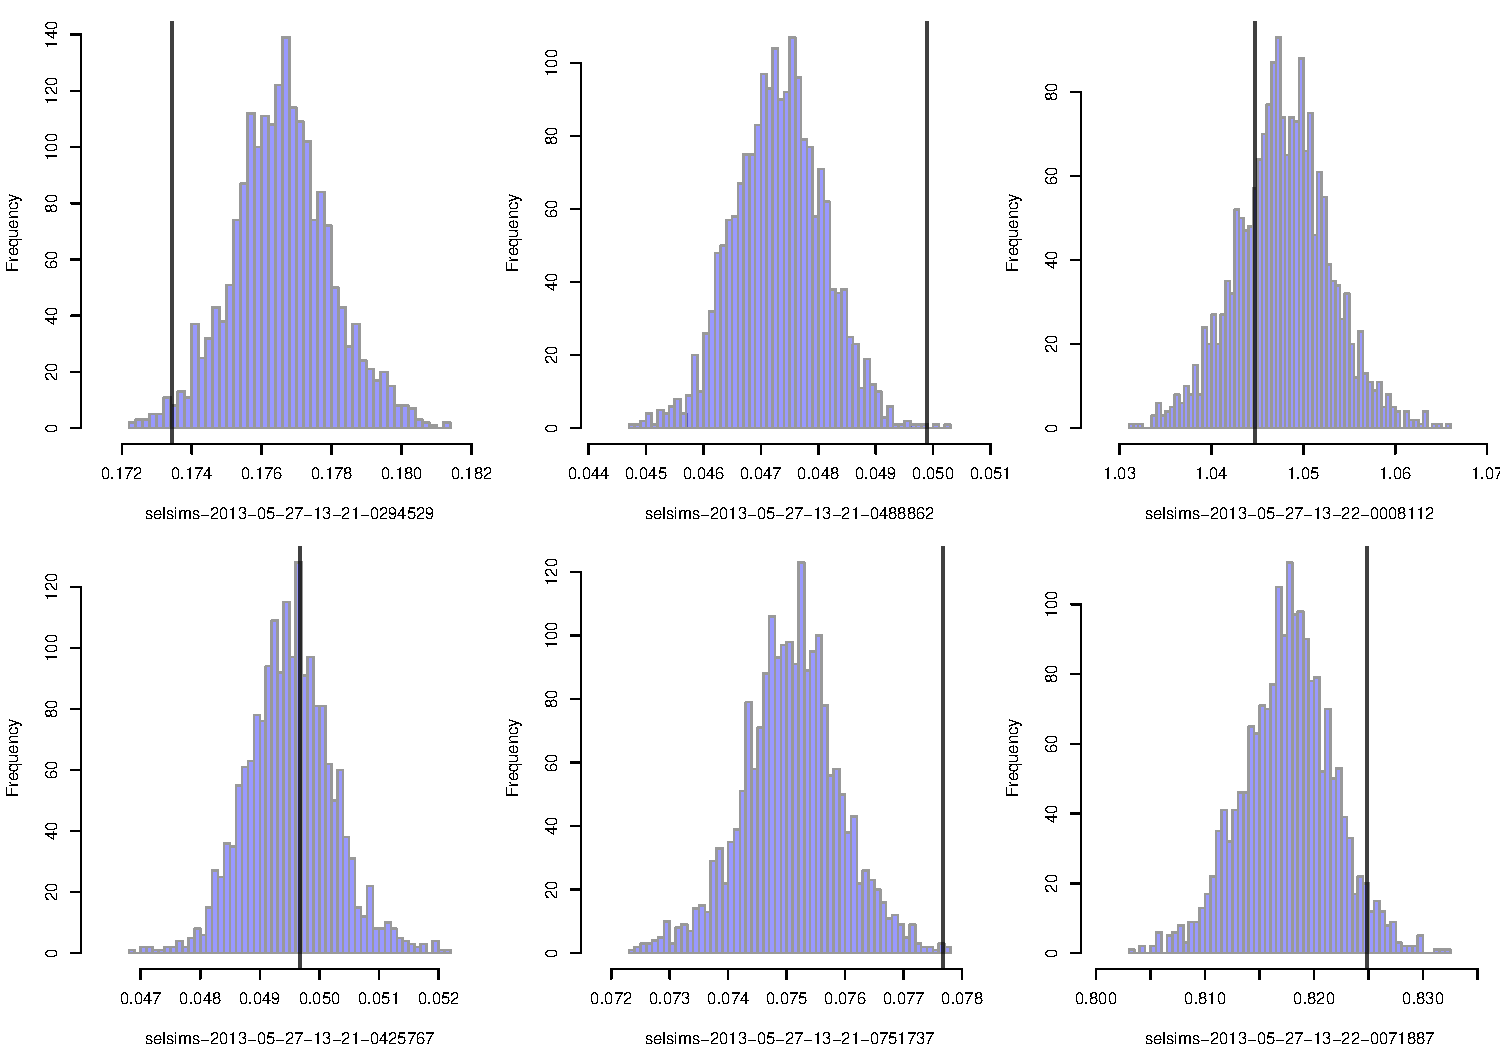
\includegraphics[width=\textwidth]{../tasep/all-mcmc-runs}
  \end{center}
  \caption{ Results from MCMC estimates for six different data sets of the parameter in TASEP (mutation rate multiplied by time).  
  Vertical line shows the true value.
  }
\end{figure}


\subsection{Ising model}

Strings of length $10^6$ were evolved under Glauber dynamics on the Ising model with varying parameters,
and pattern occurrences counted.
As for TASEP, unning 10,000 MCMC iterations with window sizes of $\ell=w=3$ (total length 9) on these takes around 40 minutes.
In this case, the true parameter values have good distribution within the estimated posterior distributions.

Here is an example, with all parameters equal to 1, for $t=.5$:
\begin{center}
 \setlength{\tabcolsep}{0pt}
\begin{tabular}{cccccccccccccccccccccccccccccccccccccccccccccccccccccccccccc}
X&X&O&X&X&O&O&X&O&X&O&X&X&O&O&X&O&O&O&O&X&X&X&O&X&O&X&O&X&O&O&O&X&X&O&X&X&X&X&X&O&X&O&X&O&X&X&X&X&O&O&X&X&X&X&X&X&O&O&O \\
x&x&o&x&X&X&O&x&o&x&$\centerdot$&x&x&O&X&X&$\centerdot$&O&X&O&X&x&x&o&x&o&x&o&x&O&X&O&$\centerdot$&$\centerdot$&O&O&X&X&O&X&X&X&o&x&o&$\centerdot$&X&O&X&o&o&x&X&X&X&O&X&o&$\centerdot$&$\centerdot$ 
\end{tabular}
\end{center}
The notation is as above; except that the entire matched pattern involved in a change is uppercase:
to simulate, we look in windows of size 3; so if XOO changes to XXO, the whole thing is uppercase, not just the middle X.

\begin{figure}
  \begin{center}
    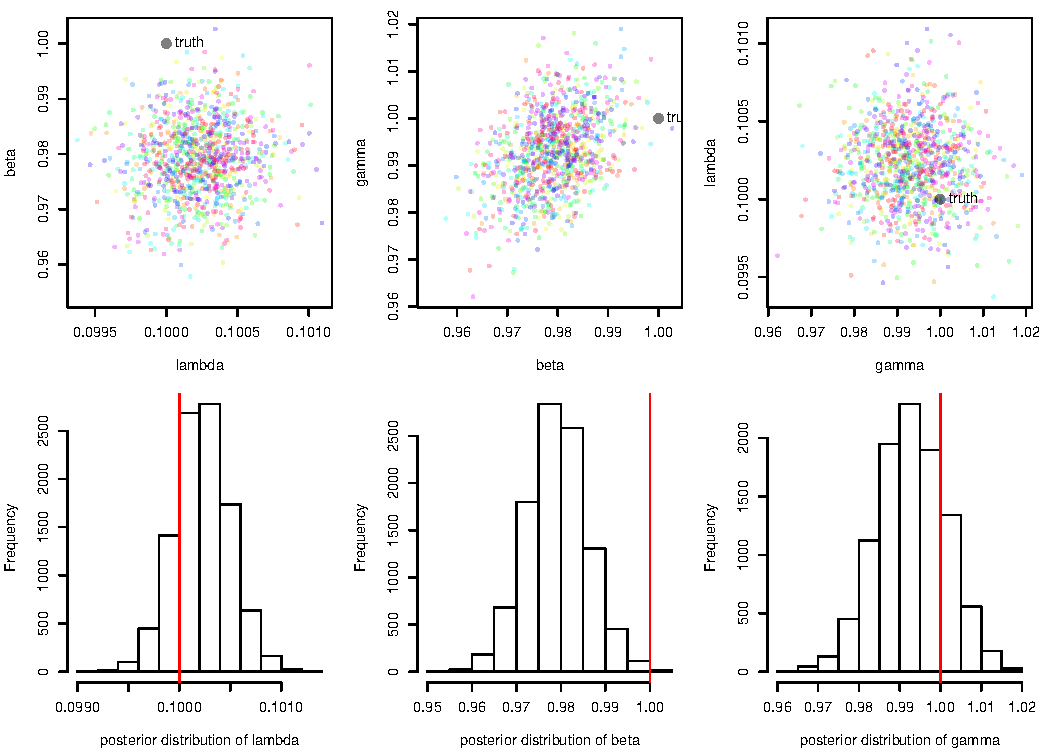
\includegraphics{../writeup-plots/selsims-2013-05-28-17-12-0275615-traces}
  \end{center}
  \caption{ 
  MCMC traces of the parameters in the Ising model across 100,000 iterations.
  The units of $\lambda$ are in mean number of changes per site.
  Vertical line shows the true value.
  }
\end{figure}

\begin{figure}
  \begin{center}
    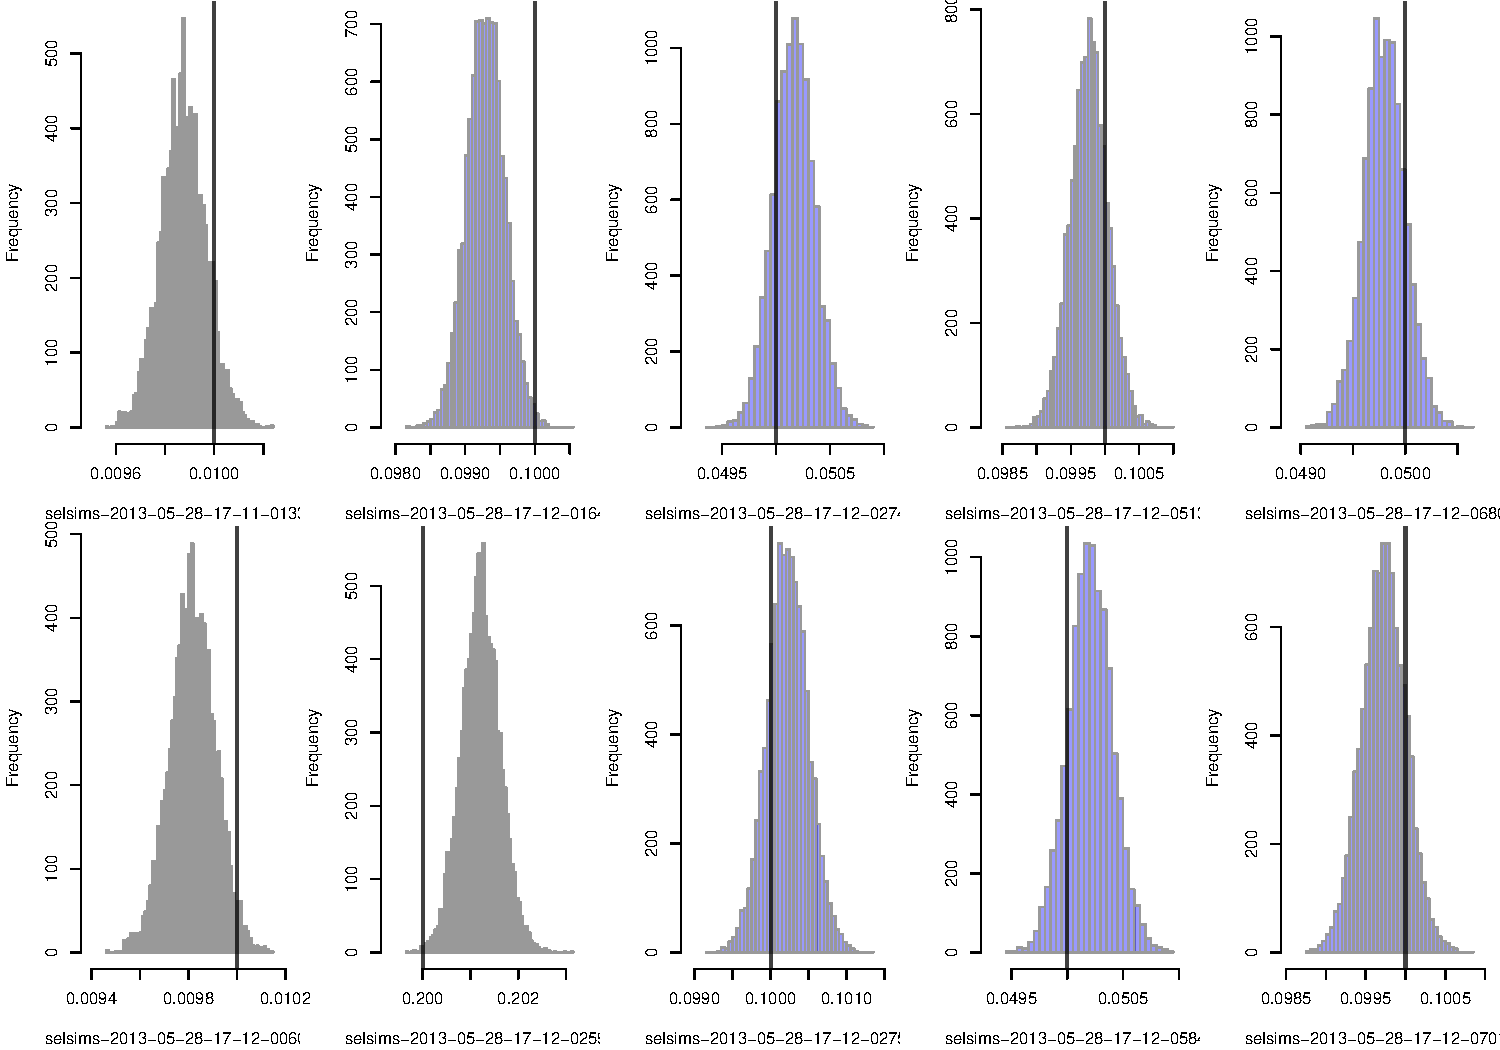
\includegraphics[width=\textwidth,page=1]{../ising/all-mcmc-runs}
  \end{center}
  \caption{ Results from MCMC estimates of the time-scaled mutation rate parameter $\lambda t$,
  in ten different simulated datasets under the Ising model.
  Vertical line shows the true value.
  }
\end{figure}

\begin{figure}
  \begin{center}
    \includegraphics[width=\textwidth,page=2]{../ising/all-mcmc-runs}
  \end{center}
  \caption{ Results from MCMC estimates of the inverse temperature $\beta$ in the Ising model. 
  Vertical line shows the true value.
  }
\end{figure}

\begin{figure}
  \begin{center}
    \includegraphics[width=\textwidth,page=3]{../ising/all-mcmc-runs}
  \end{center}
  \caption{ Results from MCMC estimates of the magnetization parameter $\beta$ in the Ising model. 
  Vertical line shows the true value.
  }
\end{figure}

%%%
\subsection{CpG mutation, on a tree}

Nucleotide sequences of length $10^6$ were simulated down two (unequal) branches of a tree,
with all single-base substitution rates $m_{xy}$ set equal (varying from a total of .01 to .1 across the tree)
and an additional CpG rate $\gamma$ set to either 0 or three times the single-base rate.
Analysis was done with $\ell=2$ and $w=1$ (a five-to-one window).

The state at the root of the tree was independently chosen bases with equal frequencies, 
and these frequencies at the root were added as parameters to the model (with a Dirichlet prior).

Here is a short example, with all parameters equal to 1, with each branch of the tree having length $0.1$:
\begin{center}
 \setlength{\tabcolsep}{0pt}
\begin{tabular}{cccccccccccccccccccccccccccccccccccccccccccccccccccccccccccc}
T&G&G&A&G&A&G&G&T&C&T&G&C&C&A&T&A&G&A&C&G&G&G&C&G&C&C&G&C&C&T&A&G&G&A&G&C&C&G&C&G&T&T&T&T&G&C&G&T&G&G&T&G&T&T&G&T&G&G&C \\
$\centerdot$&$\centerdot$&g&C&G&a&$\centerdot$&$\centerdot$&$\centerdot$&$\centerdot$&T&A&C&A&$\centerdot$&$\centerdot$&$\centerdot$&T&A&T&$\centerdot$&$\centerdot$&$\centerdot$&T&G&c&C&C&A&C&$\centerdot$&$\centerdot$&$\centerdot$&$\centerdot$&$\centerdot$&$\centerdot$&$\centerdot$&$\centerdot$&$\centerdot$&G&G&G&t&A&T&$\centerdot$&$\centerdot$&G&A&g&C&G&$\centerdot$&$\centerdot$&$\centerdot$&$\centerdot$&t&T&G&A \\
$\centerdot$&$\centerdot$&$\centerdot$&$\centerdot$&$\centerdot$&$\centerdot$&$\centerdot$&A&T&$\centerdot$&$\centerdot$&$\centerdot$&$\centerdot$&$\centerdot$&$\centerdot$&T&T&G&T&$\centerdot$&$\centerdot$&G&A&T&$\centerdot$&$\centerdot$&$\centerdot$&G&G&c&t&A&A&G&C&$\centerdot$&$\centerdot$&$\centerdot$&G&T&G&A&t&t&t&g&$\centerdot$&$\centerdot$&$\centerdot$&$\centerdot$&$\centerdot$&$\centerdot$&G&A&$\centerdot$&$\centerdot$&$\centerdot$&$\centerdot$&A&C 
\end{tabular}
\end{center}
Top is ancestral sequence (``unobserved''); bottom two are at the tips.

The point estimates are good, 
as are the MCMC estimates,
but there seems to be mixing trouble having to do with the root frequencies.

\begin{figure}
  \begin{center}
    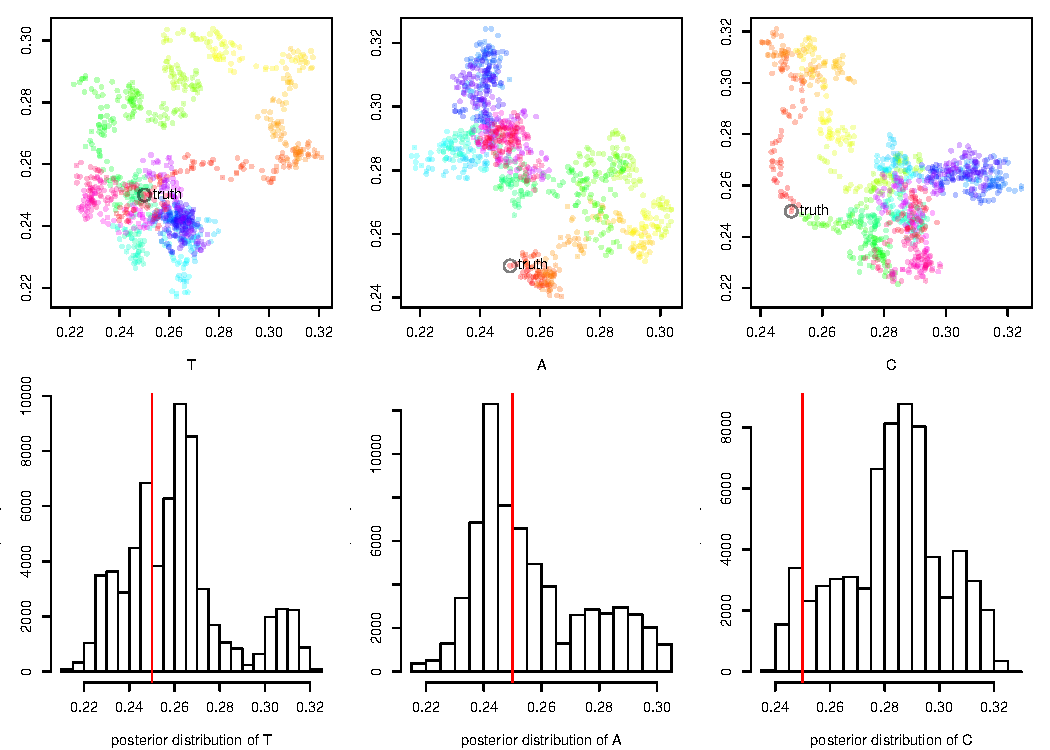
\includegraphics{../writeup-plots/selsims-2013-06-03-13-17-0790276-initfreqs}
  \end{center}
  \caption{ 
  MCMC traces across 660,000 iterations of the frequencies at the root of the (two-taxon) tree in the CpG model.
  Vertical line shows the true value.
  }
\end{figure}

\begin{figure}
  \begin{center}
    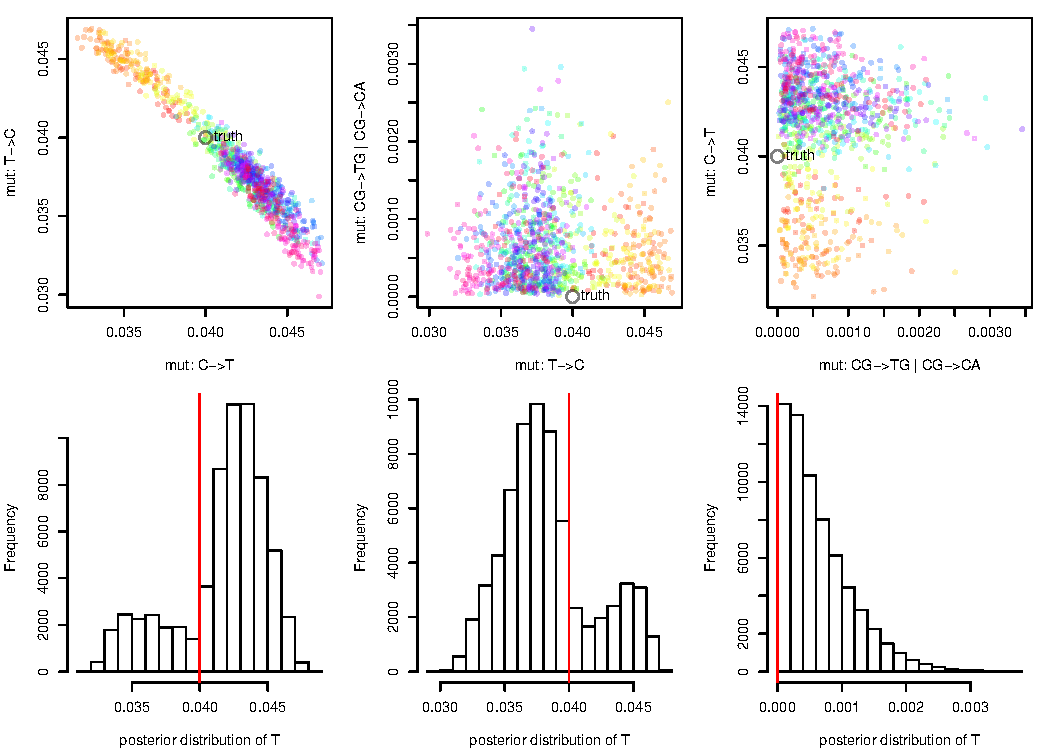
\includegraphics{../writeup-plots/selsims-2013-06-03-13-17-0790276-mutrates}
  \end{center}
  \caption{ 
  MCMC traces across 660,000 iterations of several mutation rate parameters in the CpG model.
  Units are in mean number of substitutions per base across the entire tree.
  Vertical line shows the true value.
  }
\end{figure}

%%%%%%%%
\section{Power sims}

Assess power and accuracy in the Ising model, by running replicates at these parameters:

\begin{tabular}{|rlllrrr|}
  \hline
  seqlen   &  $\lambda t$   &  $\beta$  &  $\gamma$  &  $w$ &  $\ell$   & \# reps \\
  \hline
  $10^4$    &   .2  &   1   &   .5  &   3   &   3   &   10  \\
  $10^3$    &   .2  &   1   &   .5  &   3   &   3   &   10  \\
  $10^2$    &   .2  &   1   &   .5  &   3   &   3   &   10  \\
  \hline
  $10^4$    &   .4  &   1   &   .5  &   3   &   3   &   10  \\
  $10^4$    &   .1  &   1   &   .5  &   3   &   3   &   10  \\
  $10^4$    &   .05  &   1   &   .5  &   3   &   3   &   10  \\
  \hline
  $10^4$    &   .2  &   1   &   0  &   3   &   3   &   10  \\
  \hline
  $10^4$    &   .2  &   1   &   .5  &   3   &   2   &   10  \\
  $10^4$    &   .2  &   1   &   .5  &   3   &   1   &   10  \\
  $10^4$    &   .2  &   1   &   .5  &   3   &   0   &   10  \\
  \hline
\end{tabular}

\section{Applications}

graham:
\begin{itemize}

\item estimating freq spectrum [Hernandez]

\item probabilistic ancestral states for common ancestor of e.g. humans 4N generations ago [Siepel] -- would widely used for primates

\end{itemize}


%%%%%%%%
\section{What next}

\begin{enumerate}

  \item Allow more than single-base distribution at the root.

  \item What's up with the mixing problem in root frequencies?

  \item See if counting in nonoverlapping windows fixes the peakiness problem with TASEP. \emph{Yes, it does.}

  \item See what's feasible with a larger alphabet -- 60 codons -- and more parameters.

  \item Show that taking no context ($\ell=0$) can be positively misleading in some context.

  \item Do a three-taxa tree.

  \item How to identify motifs in the residuals?

\end{enumerate}

\end{document}
